\documentclass{article}

\usepackage{fancyhdr} % Required for custom headers
\usepackage{lastpage} % Required to determine the last page for the footer
\usepackage{extramarks} % Required for headers and footers
\usepackage[usenames,dvipsnames]{color} % Required for custom colors
\usepackage[table]{xcolor}
\usepackage{graphicx} % Required to insert images
\usepackage{listings} % Required for insertion of code
\usepackage{algpseudocode} % Required for pseudocode listing
\usepackage{courier} % Required for the courier font
\usepackage{amsmath}
\usepackage{amssymb}
\usepackage{booktabs}
\usepackage{multirow}
\usepackage{tikz}
\usetikzlibrary{arrows, shapes, positioning, calc}
\usepackage{caption}
\usepackage{wasysym}
\usepackage{multirow}
\usepackage{float}
\usepackage{tcolorbox}
\usepackage{csquotes}
\usepackage{fancybox}
\usepackage{enumitem}
\usepackage[letterspace=150]{microtype}
\usepackage{cancel}

% Margins
\topmargin=-0.45in
\evensidemargin=0in
\oddsidemargin=0in
\textwidth=6.5in
\textheight=9.0in
\headsep=0.25in

\linespread{1.1} % Line spacing

% Set up the header and footer
\pagestyle{fancy}
\lhead{\labAuthorName} % Top left header
\chead{\labTitle} % Top center head
\rhead{\firstxmark} % Top right header
\lfoot{\lastxmark} % Bottom left footer
\cfoot{} % Bottom center footer
\rfoot{Page\ \thepage\ of\ \protect\pageref{LastPage}} % Bottom right footer
\renewcommand\headrulewidth{0.4pt} % Size of the header rule
\renewcommand\footrulewidth{0.4pt} % Size of the footer rule

\usepackage{fancyvrb}

\setlength\parindent{0pt} % Removes all indentation from paragraphs


%----------------------------------------------------------------------------------------
%	DOCUMENT STRUCTURE COMMANDS
%	Skip this unless you know what you're doing
%----------------------------------------------------------------------------------------

% Header and footer for when a page split occurs within a problem environment
\newcommand{\enterProblemHeader}[1]{
\nobreak\extramarks{#1}{#1 continued on next page\ldots}\nobreak
\nobreak\extramarks{#1 (continued)}{#1 continued on next page\ldots}\nobreak
}

% Header and footer for when a page split occurs between problem environments
\newcommand{\exitProblemHeader}[1]{
\nobreak\extramarks{#1 (continued)}{#1 continued on next page\ldots}\nobreak
\nobreak\extramarks{#1}{}\nobreak
}

\setcounter{secnumdepth}{0} % Removes default section numbers
\newcounter{labProblemCounter} % Creates a counter to keep track of the number of problems

\newcommand{\labProblemName}{}
\newenvironment{labProblem}[1][Problem \arabic{labProblemCounter}]{ % Makes a new environment called labProblem which takes 1 argument (custom name) but the default is "Problem #"
\stepcounter{labProblemCounter} % Increase counter for number of problems
\renewcommand{\labProblemName}{#1} % Assign \labProblemName the name of the problem
\subsection{\labProblemName} % Make a section in the document with the custom problem count
\enterProblemHeader{\labProblemName} % Header and footer within the environment
}{
\exitProblemHeader{\labProblemName} % Header and footer after the environment
}

\newcommand{\problemAnswer}[1]{ % Defines the problem answer command with the content as the only argument
\noindent\framebox[\columnwidth][c]{\begin{minipage}{0.98\columnwidth}#1\end{minipage}} % Makes the box around the problem answer and puts the content inside
}

\newcommand{\labSectionName}{}
\newenvironment{labSection}[1]{ % New environment for sections within homework problems, takes 1 argument - the name of the section
\renewcommand{\labSectionName}{#1} % Assign \homeworkSectionName to the name of the section from the environment argument
\subsection{\labSectionName} % Make a subsection with the custom name of the subsection
\enterProblemHeader{\labProblemName\ [\labSectionName]} % Header and footer within the environment
}{
\enterProblemHeader{\labProblemName} % Header and footer after the environment
}

%----------------------------------------------------------------------------------------
%	NAME AND CLASS SECTION
%----------------------------------------------------------------------------------------

\newcommand{\labTitle}{Hash Function and Public Key Cryptography} % Assignment title
\newcommand{\labDueDate}{18\ November,\ 2019} % Due date
\newcommand{\labClass}{CSCE\ 465} % Course/class
\newcommand{\labClassTime}{Fall 2019} % Class/lecture time
\newcommand{\labClassInstructor}{Gu} % Teacher/lecturer
\newcommand{\labAuthorName}{M. Hunter Martin} % Your name
\newcommand{\labAuthorUIN}{825002697}

%----------------------------------------------------------------------------------------
%	TITLE PAGE
%----------------------------------------------------------------------------------------

\title{
\vspace{2in}
\textmd{\textbf{\labClass\ :\ \labTitle}}\\
\normalsize\vspace{0.1in}\small{Due\ on\ \labDueDate}\\
\vspace{0.1in}\large{\textit{\labClassInstructor\ \labClassTime}}
\vspace{3in}
}

\author{\textbf{\labAuthorName}\\ \textbf{\labAuthorUIN}}
\date{}

%----------------------------------------------------------------------------------------

\begin{document}

\maketitle
\newpage

\section{Written Problems}
\begin{labProblem}[5.2 (8 pts)]
\begin{displayquote}
\begin{tcolorbox}
Message digests are reasonably fast, but here’s a much faster function to compute. Take your message, divide it into 128-bit chunks, and $xor$ all the chunks together to get a 128-bit result. Do the standard message digest on the result. Is this a good message digest function?
\end{tcolorbox}
\end{displayquote}
No.  It would be relatively easy to find collisions and that would ruin the security of the function.

\end{labProblem}

\begin{labProblem}[5.14 (12 pts)]
\begin{displayquote}
\begin{tcolorbox}
For purposes of this exercise, we will define random as having all elements equally likely to be chosen. So a function that selects a 100-bit number will be random if every 100-bit number is equally likely to be chosen. Using this definition, if we look at the function ``+" and we have two inputs, $x$ and $y$, then the output will be random if at least one of $x$ and $y$ are random. For the following functions, find sufficient conditions for $x$, $y$ and $z$ under which the output will be random:
\end{tcolorbox}
\end{displayquote}
\subsubsection{1) $\sim x$}

If $x$ is random, $\sim x$ will also be random. $y$ and $z$ are independent.

\subsubsection{2) $x\oplus y$}

If either $x$ or $y$ are the random, and they are not equal, the output will be random. $z$ is independent.

\subsubsection{3) $x \lor y$}

If either $x$ or $y$ are the random, and they are not equal, the output will be random. $z$ is independent.

\subsubsection{4) $x\land y$}

If either $x$ or $y$ are the random, and they are not equal, the output will be random. $z$ is independent.

\subsubsection{5) $(x \land y) \lor (\sim x \land z)$ [the selection function]}

If $(x \land y)$ is non-zero, or $(\sim x \land z)$ is non-zero, the output should be random assuming at least one of the inputs is also random.

\subsubsection{6) $(x \land y) \lor (x \land z) \lor (y \land z)$ [the majority function]}

As long as either $x$, $y$, or $z$ are different, and at least one is random, then the output should also be random.

\subsubsection{7) $x\oplus y\oplus z$}

As long as at least 2 of the numbers are different (i.e. $x$ and $y$, or $x$ and $z$, etc.) and at least one of the unique numbers is random, the output will be random.

\subsubsection{8) $y\oplus (x\lor \sim z)$}

If $(x\lor \sim z) \neq y$, the output will be random if at least one of the numbers is random.

\end{labProblem}

\begin{labProblem}[6.2 (8 pts)]
\begin{displayquote}
\begin{tcolorbox}
In the KPS textbook, it states that encrypting the Diffie-Hellman value with the other side’s public key prevents the man-in-the-middle attack. Why is this the case, given that an attacker can encrypt whatever it wants with the other side’s public key?
\end{tcolorbox}
\end{displayquote}
The main point of Public-Key Encryption is for private key distribution.  The Private key is needed the decrypt the Diffie-Hellman value, so the Man-in-the-Middle won't be able to decrypt the key.

\end{labProblem}

\begin{labProblem}[6.8 (8 pts)]
\begin{displayquote}
\begin{tcolorbox}
Suppose Fred sees your RSA signature on $m_1$ and on $m_2$ (i.e., he sees $m^d_1$ mod $n$ and $m^d_2$ mod $n$). How does he compute the signature on each of $m^j_1$ mod $n$ (for positive integer $j$), $m^{-1}_1$ mod $n$, $m_1m_2$ nod $n$, and in general $m^j_1m^k_2$ mod $n$ (for arbitrary integers $j$ and $k$)?
\end{tcolorbox}
\end{displayquote}

\subsubsection{$m^j_1$ mod $n$ (for positive integer $j$)?}

$\textmd{Signature } = (m_1^d)^j$ mod $n = (m_1^j)^d$ mod $n$

\subsubsection{$m^{-1}_1$ mod $n$?}

$\textmd{Signature } = (m_1^d)^{-1}$ mod $n = (m_1^{-1})^d$ mod $n$

\subsubsection{$m_1m_2$ mod $n$?}
$\textmd{Signature } =(m_1m_2)^d$ mod $n = (m_1^d$ mod $n)(m_2^d$ mod $n)$ mod $n$.

\subsubsection{$m^j_1m^k_2$ mod $n$ (for arbitrary integers $j$ and $k$)?}
$\textmd{Signature } =(m_1^jm_2^k)^d$ mod $n = (m_1^d$ mod $n)^j(m_2^d$ mod $n)^k$ mod $n$.


\end{labProblem}

\section{Task 1: Generating Message Digest and MAC [7 pts]}
The following is my input.txt.
\begin{verbatim}
The FitnessGram Pacer Test is a multistage aerobic capacity test
that progressively gets more difficult as it continues. The 20
meter pacer test will begin in 30 seconds. Line up at the start.
The running speed starts slowly, but gets faster each minute after
you hear this signal. [beep] A single lap should be completed each
time you hear this sound. [ding] Remember to run in a straight
line, and run as long as possible. The second time you fail to
complete a lap before the sound, your test is over. The test will
begin on the word start. On your mark, get ready, start.
\end{verbatim}

\subsection{MD5 Message Digest}
\begin{center}
    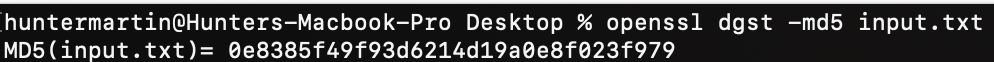
\includegraphics[scale=0.75]{md5-task1.png}
\end{center}

The hash function generated a hash from my input.  The hash was somewhat short.

\subsection{SHA1 Message Digest}
\begin{center}
    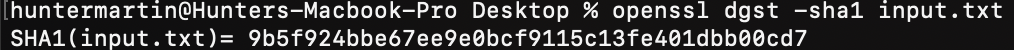
\includegraphics[scale=0.75]{sha1-task1.png}
\end{center}

The hash function generated a hash from my input.  The hash was somewhat short, but longer than the MD5 hash.  This is likely part of what makes this hash function more secure than the MD5 hash.

\subsection{SHA256 Message Digest}
\begin{center}
    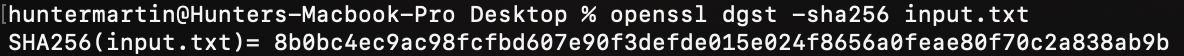
\includegraphics[scale=0.75]{sha256-task1.png}
\end{center}

The hash function generated a hash from my input.  The hash was much longer than the MD5, and somewhat longer than the SHA1, which probably explains why it's considered so much more secure.

\section{Task 2: Keyed Hash and HMAC [9 pts]}
The following is my input.txt.
\begin{verbatim}
The FitnessGram Pacer Test is a multistage aerobic capacity test
that progressively gets more difficult as it continues. The 20
meter pacer test will begin in 30 seconds. Line up at the start.
The running speed starts slowly, but gets faster each minute after
you hear this signal. [beep] A single lap should be completed each
time you hear this sound. [ding] Remember to run in a straight
line, and run as long as possible. The second time you fail to
complete a lap before the sound, your test is over. The test will
begin on the word start. On your mark, get ready, start.
\end{verbatim}

\subsection{MD5 Hash}
\begin{center}
    MD5 Hash with the standard key,
    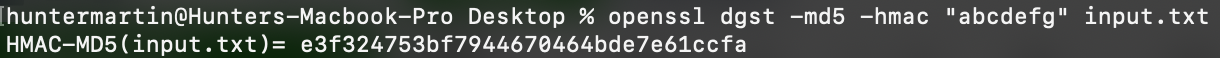
\includegraphics[scale=0.65]{md5-1-task2.png}
    
    and again with an extended key.
    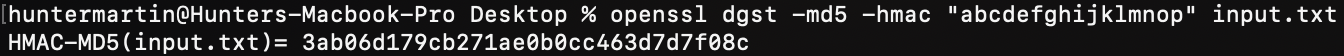
\includegraphics[scale=0.65]{md5-2-task2.png}
\end{center}

\subsection{SHA1 Hash}
\begin{center}
    SHA1 Hash with the standard key,
    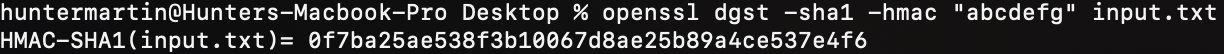
\includegraphics[scale=0.65]{sha1-1-task2.png}
    
    and again with an extended key.
    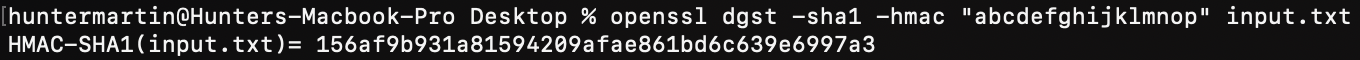
\includegraphics[scale=0.65]{sha-2-task2.png}
\end{center}

\subsection{SHA256 Hash}
\begin{center}
    SHA256 Hash with the standard key,
    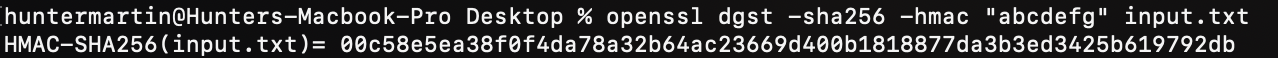
\includegraphics[scale=0.65]{sha256-1-task2.png}
    
    and again with an extended key.
    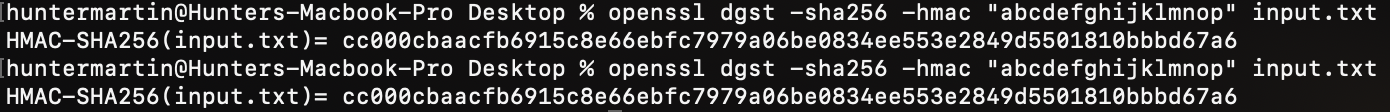
\includegraphics[scale=0.65]{sha256-2-task2.png}
\end{center}

The keys didn't seem to affect the length of the final output, and the output was consistent between runs.  This leads me to believe that the Key Size did not affect the hash, and a fixed key is not required.

\section{Task 3: The Randomness of One-way Hash [9 pts]}
\begin{center}
    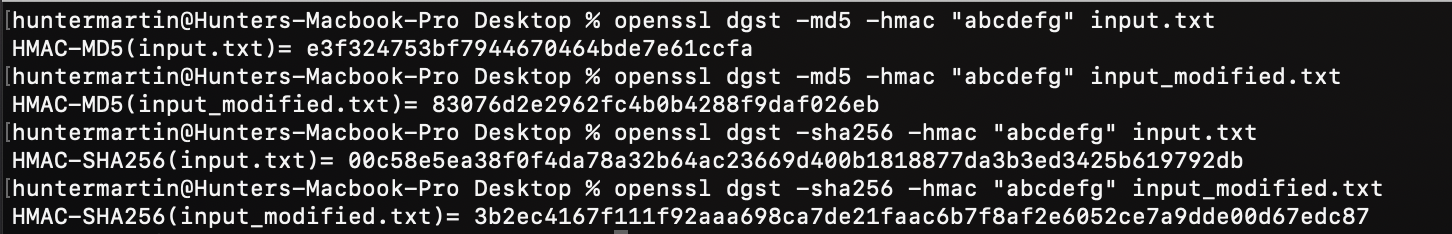
\includegraphics[scale=0.6]{task3.png}
\end{center}

The difference between the two  with respect to each hash type is obvious.  When we flipped even just one bit in the input, the entire output is totally different.  This demonstrates out even a small change in the input generates a totally different output with these secure hashes.

\section{Task 4: Hash Collision-Free Property [20+10 bonus pts]}
\begin{center}
    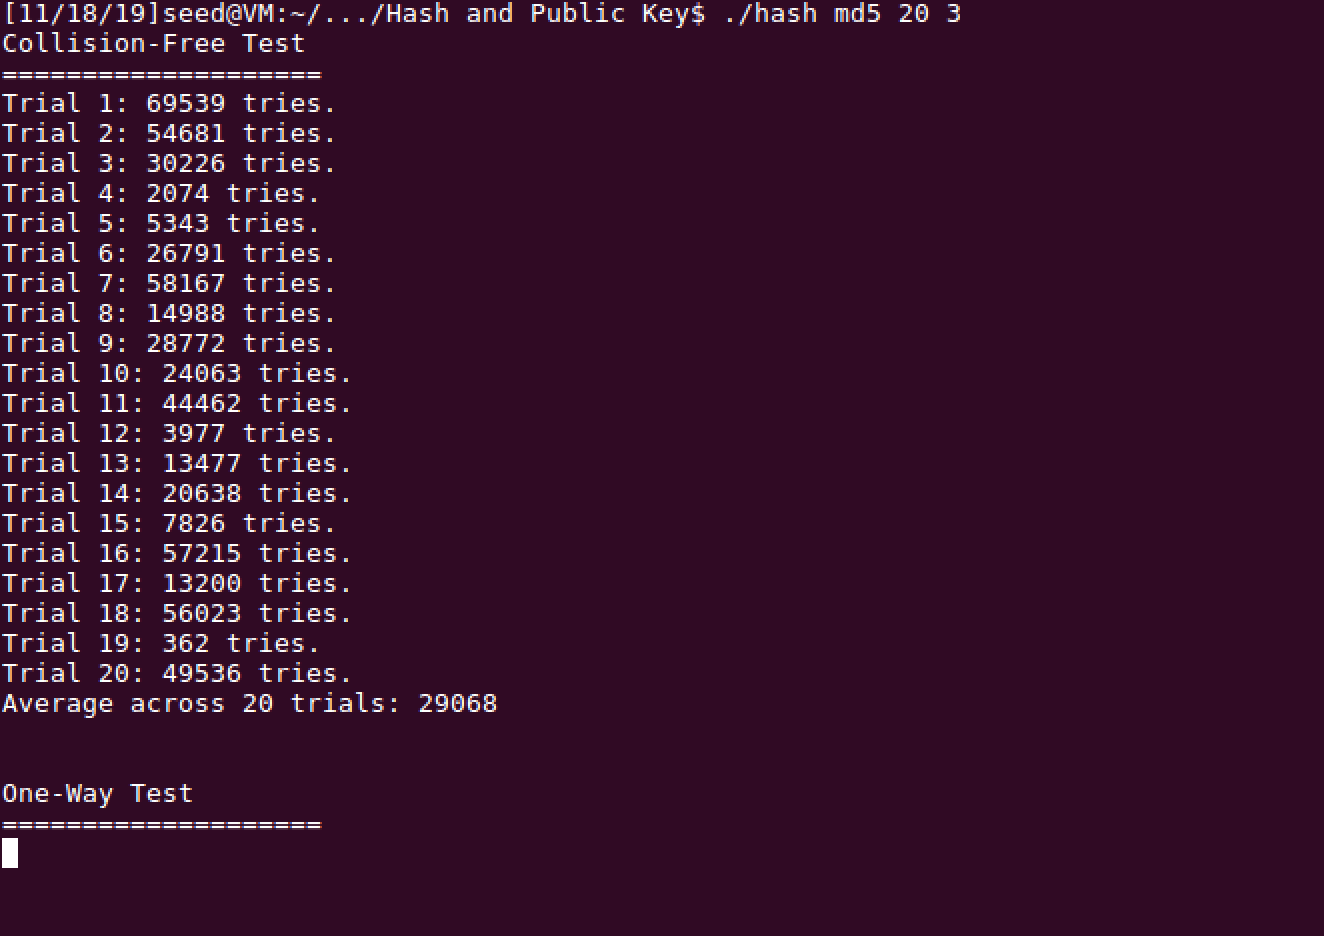
\includegraphics[scale=0.5]{task4.png}
\end{center}

The average in the first test took about 29068 tries on average, with a maximum near 70000, and a minimum of 362.  The average of the one-way test was much higher, well into the hundreds of millions of tries.  My implementation does work, but takes a very long time to find a collision.  This is a testament to just how difficult it is to find a specific collision.  Finding any collision is easy, but a specific one is very difficult.

\subsection{Proof of the Difference (+10 bonus points)}
The proof of this is similar to what we call \textit{the Birthday Paradox.} In the Birthday Paradox, we can prove than in a classroom of 23 students, there is a 50-50 chance that \textit{a student} will have the same birthday as \textit{some other student}.  With 75 students, there will be a 99.97\% chance of this collision occurring.  This is true because we consider the chance that every single student has a birthday in common with every other student.  The odds in each are low, but when you have to multiply the inverse of each of these odds together, we eventually get a relatively good chance, and with only a few more students, we can all but guarantee a collision will occur.\\

This same paradox holds to hash function collisions.  In the test for finding just any collision, we found them relatively quickly, with only 30000 tries on average, but in the specific hash (one-way) collision, it's much harder.  We are only going to have an astronomically low chance each time we try.  The average was well into the hundreds of millions.  In the below test, I simulated the easier collision problem by giving up and retrying after 100,000 tries.
\begin{center}
    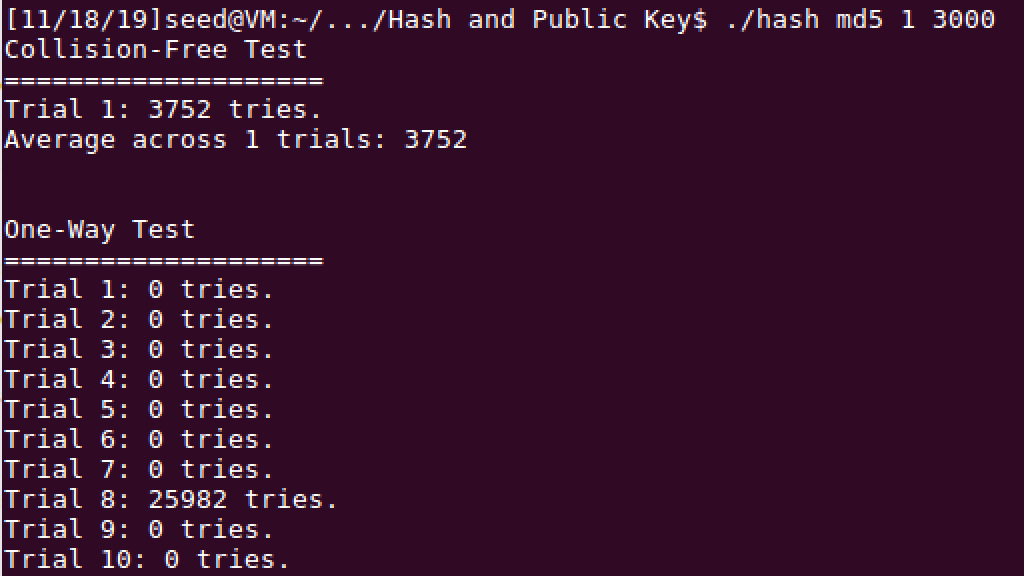
\includegraphics[scale=0.5]{task4_one_way.png}
\end{center}

We again see the lower level.  The birthday paradox is great for finding just a collision, but luckily the security is achieved with a \textit{specific} hash, so our hashes remain safe with their super-low chance of being collided with.

\section{Task 5: Performance Comparison: RSA versus AES [8 pts]}

\subsection{RSA}
\begin{center}
    \textbf{Encrypting...}\\
    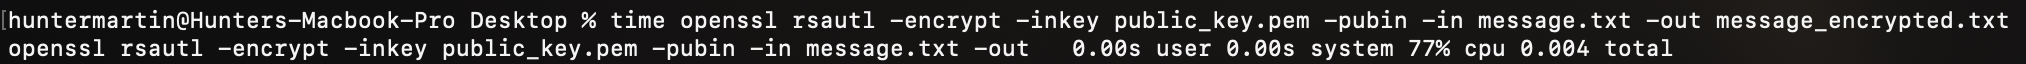
\includegraphics[scale=0.4]{rsa_in.png}
    
    \textbf{Decrypting...}\\
    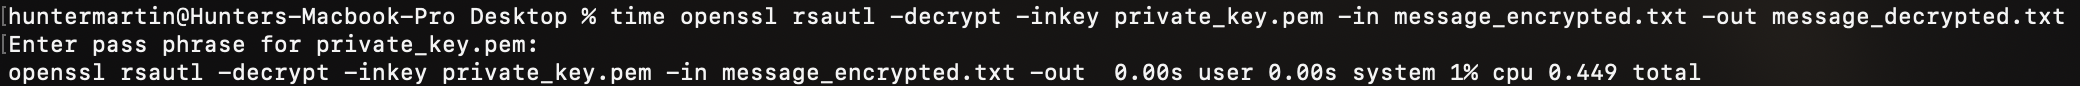
\includegraphics[scale=0.4]{rsa_out.png}
    
    \textbf{Bench-marking...}\\
    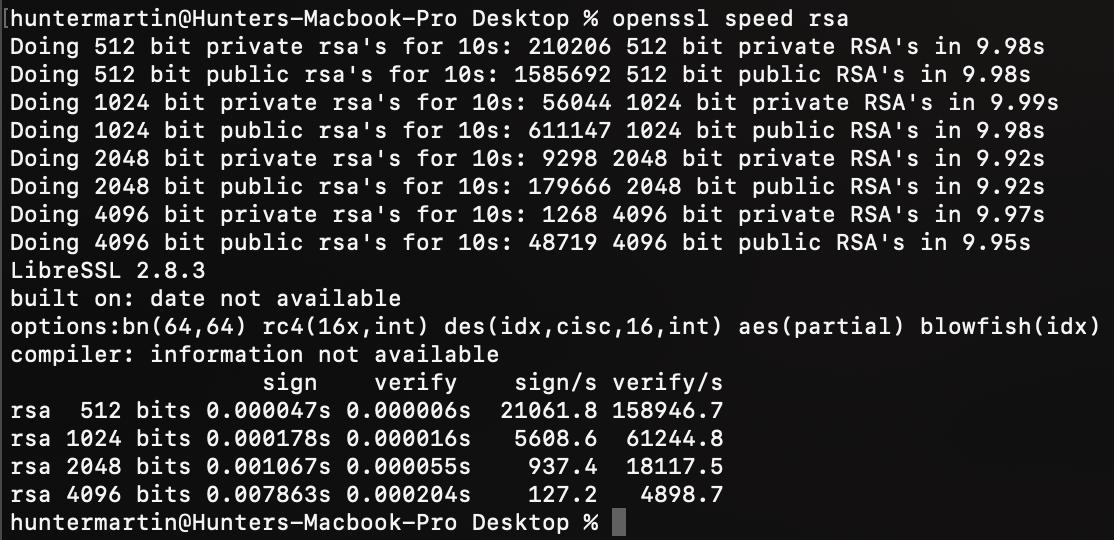
\includegraphics[scale=0.5]{rsa_benchmark.png}
\end{center}
During the individual tests, the encryption and decryption occured very quickly, but decryption did seem to take a bit longer.\\

During bench-marking, we can see that the average speed for an RSA operation is dependent on both the size of the key (shorter keys are much faster), and public is always much faster than private.

\subsection{AES}
\begin{center}
    \textbf{Encrypting...}\\
    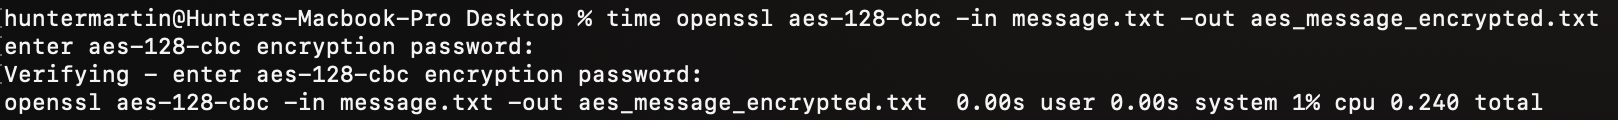
\includegraphics[scale=0.4]{aes_in.png}
    
    \textbf{Bench-marking...}\\
    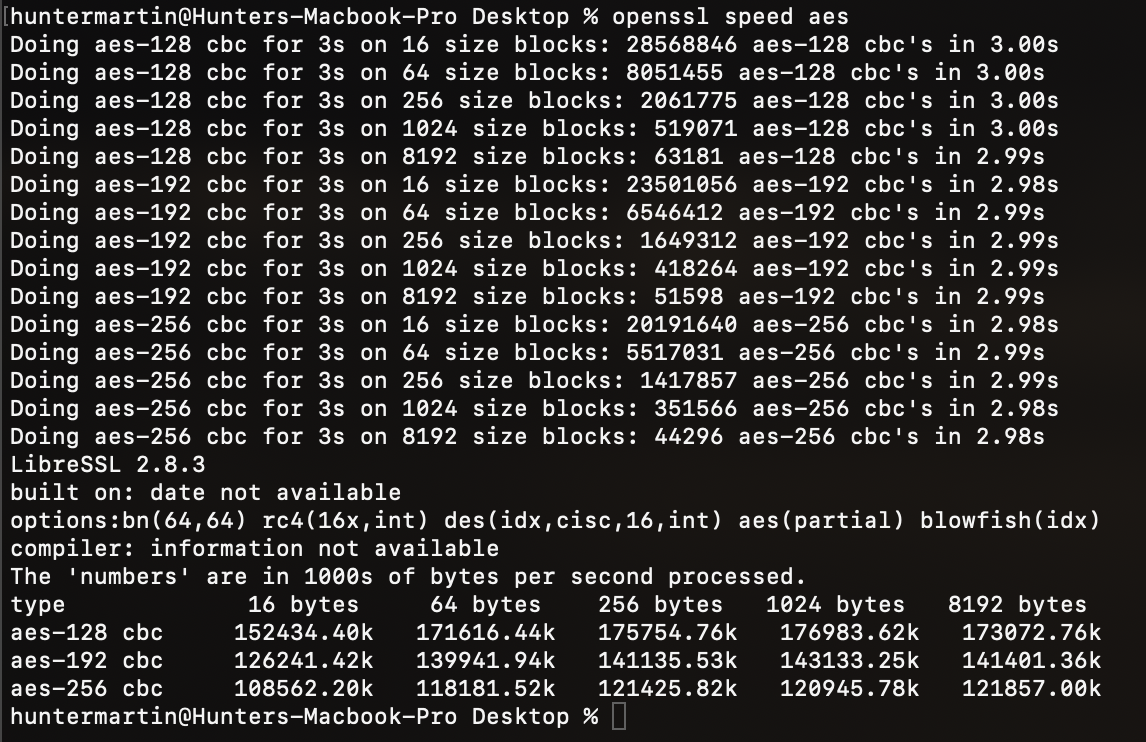
\includegraphics[scale=0.5]{aes_benchmarking.png}
\end{center}
As we noted with the RSA encryption, the speed was really too fast to measure for encryption, likely only a few hundredths of a second.\\

During bench-marking, we noticed encryption does seem to occur faster than with RSA, but is still highly dependent on the key size and on the block-size.  The larger the blocks and the larger the key, the fewer encryptions we can do in our 3 seconds.

\section{Task 6: Create Digital Signature [7 pts]}
\begin{center}
    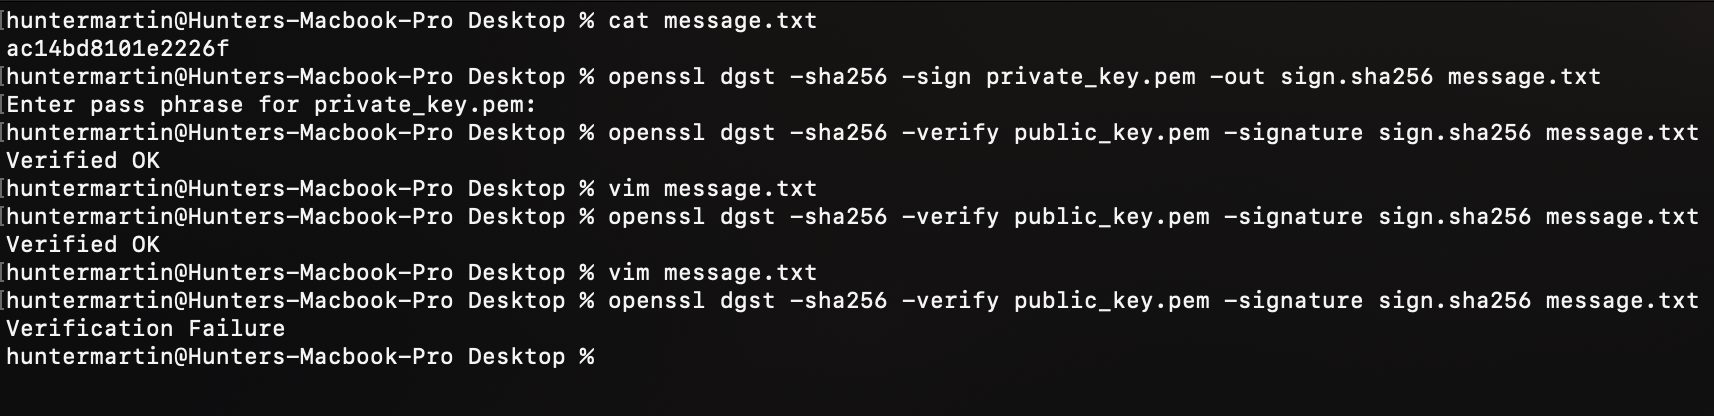
\includegraphics[scale=0.5]{task6.png}
\end{center}

Digital signatures can ensure that the message you're receiving hasn't been tampered with on the way to its destination.  Even a slight change will cause the verification to fail.  In the above screenshot, you can see that I create a signature from my own private key, then my friend can verify my message with my public key, effectively blocking the Man-in-the-middle attack.  While it wouldn't be a solution to stopping the man-in-the-middle from reading my message, I could stop him from changing my message.

\section{Attachments}
[1] \texttt{task4.c} - C code for hash collisions.  Usage will be printed when ran without arguments.\\

\textit{All pictures included in this report are also included in the Report/Source folder in the submission.}

\bibliographystyle{abbrv}
\begin{thebibliography}{9}
\bibitem{assn}
Gu.
\textmd{Homework 5: Hash Function and Public Key Cryptography.}
\bibitem{openssl}
Openssl. \textmd{https://www.openssl.org/docs/manmaster/man3/EVP\_DigestInit.html}
\end{thebibliography}

\end{document}